\documentclass{beamer}

\usepackage{amsmath}
\usepackage{amssymb}
\usepackage{graphicx}
\usepackage{indentfirst}
\usepackage{hyperref}
\usepackage{subcaption}

\graphicspath{{../../imgs}}
\usetheme{Madrid}


\author{Kainã Alves Tureso}
\title{Simulação numérica de gotas suspensas}
\date{\today}
\institute{ICMC-USP}


\begin{document}

\frame{\titlepage}
\frame{
    \tableofcontents
}

\section{Encontrando gotas}
\begin{frame}{Encontrando gotas}
    Dados $A, B \in \mathbb{R}$, resolvemos o PVI
    \[
        u'(s) = \begin{bmatrix}
            r'(s) \\ z'(s) \\ \theta'(s) \\ V'(s) \\ S'(s)
        \end{bmatrix} = \begin{bmatrix}
            \cos(\theta) \\
            \sin(\theta) \\
            A - Bz - \frac{\sin(\theta)}{r} \\
            \pi r^2 \sin(\theta)  \\
            2\pi r
        \end{bmatrix} = f(u)
    \]

    Com condições iniciais
    \[
        \begin{bmatrix}
            r \\ z \\ \theta \\ V \\ S
        \end{bmatrix} (0) = \vec{0}
    \]
\end{frame}

\begin{frame}{Encontrando gotas}
    Note que, para $r = 0$, a expressão da derivada de $\theta$ apresenta uma singularidade. Para resolver isso, está sendo utilizada uma aproximação de ordem $O(\varepsilon^4)$ para $f(u)$. Calculamos $f(u(\varepsilon = 10^{-7}))$ e usamos esse resultado como ponto inicial para o método de resolução do PVI, no caso, RK4 clássico. A aproximação é dada por:
    \[
        f(u(\varepsilon)) \approx \begin{bmatrix}
            \varepsilon - \frac{A^2}{24}\varepsilon^3 \\
            \frac{A}{4} \varepsilon^2 \\
            \frac{A}{2} \varepsilon - \frac{AB}{16} \varepsilon^3\\
            \frac{\pi A}{8}\varepsilon^4 \\
            \pi \varepsilon^2
        \end{bmatrix}
    \]
\end{frame}

\begin{frame}{Interseção com o bocal}
    Como resultado, obtemos as coordenadas dos pontos da gota, que são organizados em dois vetores: $r$ e $z$, tal que $(r_i,z_i)$ formam um ponto. Basta agora encontrar a interseção com o bocal com raio $a$. Isso é feito encontrando os argumentos $i$ e $i+1$ tal que $\min\{r_i, r_{i+1}\} \le a < \max\{r_i, r_{i+1}\}$ e fazendo a interpolação linear:
    \[
        \xi r_i + (1-\xi)r_{i+1} = a \implies \xi = \frac{a - r_{i+1}}{r_i - r_{i+1}}
    \]
    Com $\xi \in [-1,1]$.
\end{frame}


\section{Comportamento das gotas}

\begin{frame}
    Agora que conseguimos encontrar as gotas, podemos analisar qualitativamente o problema, de forma a entendê-lo melhor. A figura \ref{fig:plots} mostra alguns plots com $B=0.134752747253$ 

    \begin{figure}
        \centering
        \begin{subfigure}[b]{0.4\textwidth}
            \centering
            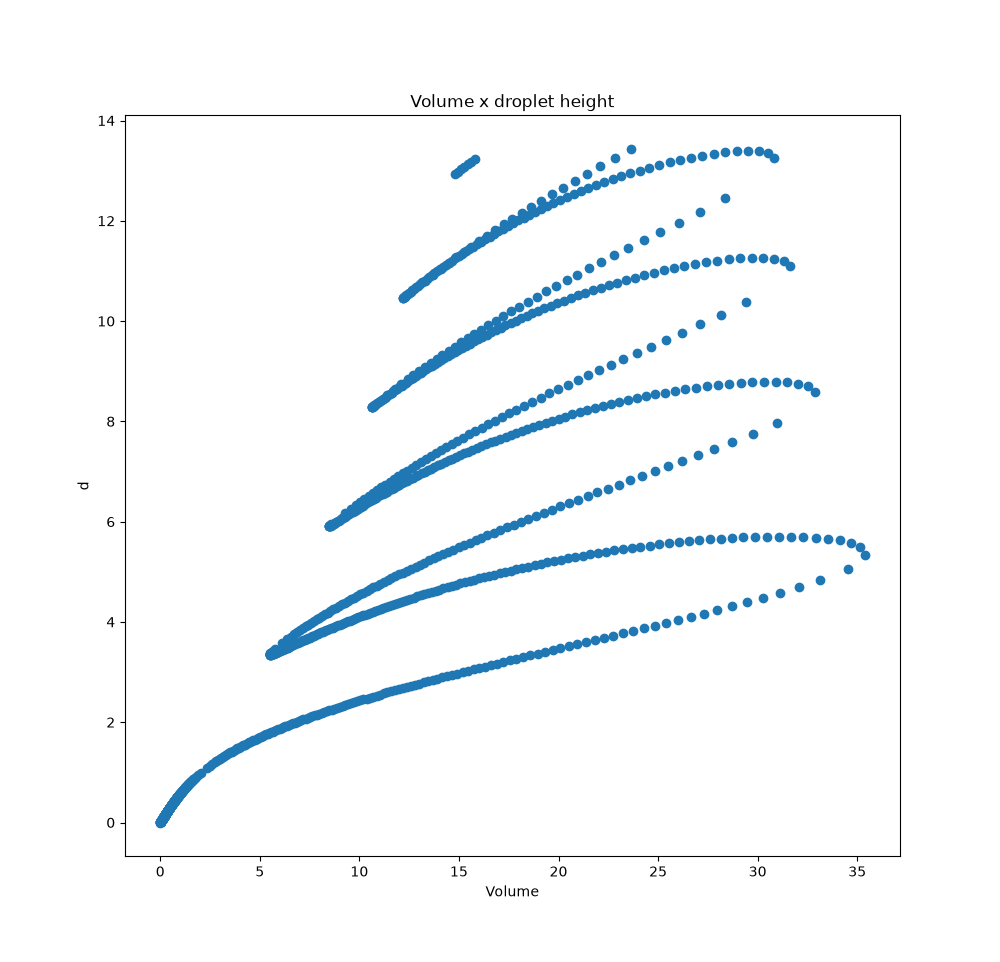
\includegraphics[width=\textwidth]{Volume_x_droplet_height.png}
            \caption{Volume da gota com relação à sua altura (adimensional)}
        \end{subfigure}
        \quad
        \begin{subfigure}[b]{0.4\textwidth}
            \centering
            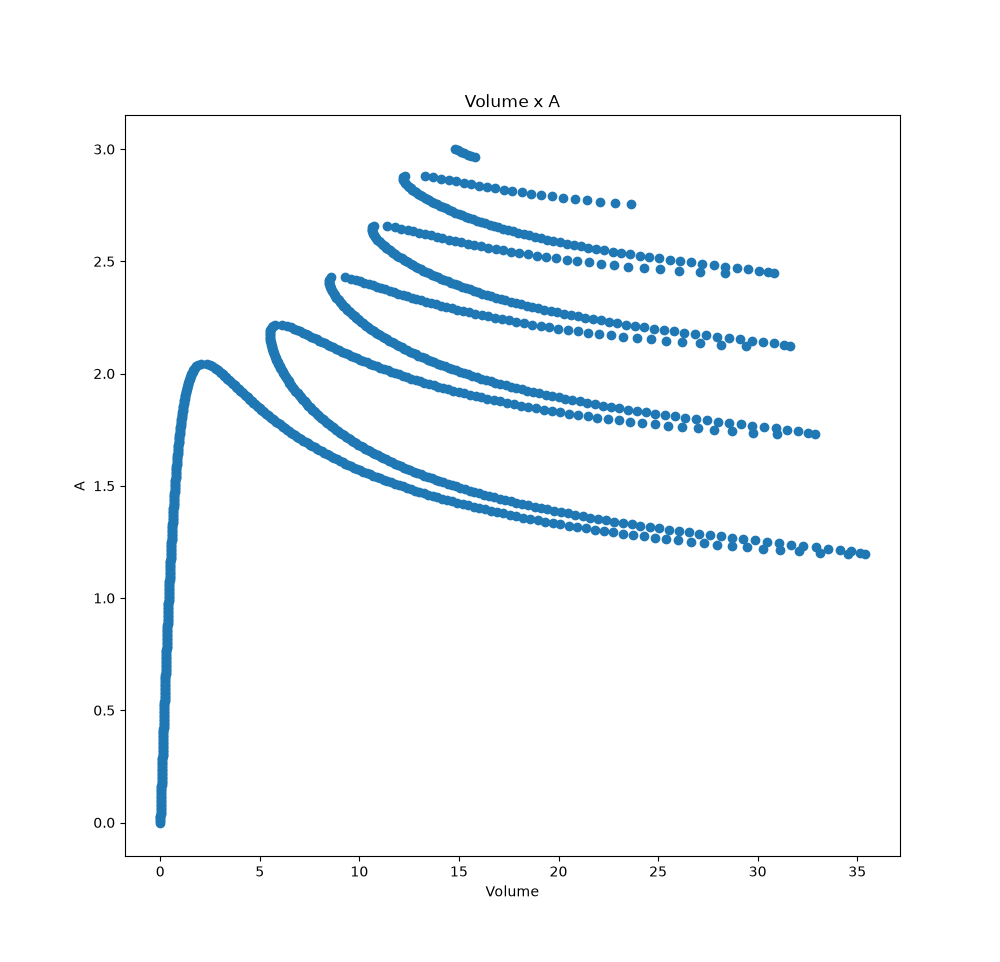
\includegraphics[width=\textwidth]{Volume_x_A.png}
            \caption{Pressão inicial com relação ao volume da gota (adimensional)}
        \end{subfigure}
        \caption{Plots qualitativos}
        \label{fig:plots}
    \end{figure}
\end{frame}

\begin{frame}
    O gráfico da pressão inicial pela pressão é o mais importante de ser analisado. Ele nos mostra quais são os ponto de Volume máximo de uma gota estável (Resultado de Maddocks) e qual a pressão máxima inicial que é fisicamente viável. \pause Como podemos encontrar esses pontos quantitativamente?
\end{frame}

\begin{frame}{Volume máximo $V^*$}
    Note que, ao limitar o valor de $A$, podemos restrigir os valores de V encontrados aos valores próximos do fim do primeiro ramo. Com isso, podemos fazer uma busca ternária para encontrar o volume máximo $V^*$
    \begin{figure}
        \centering
        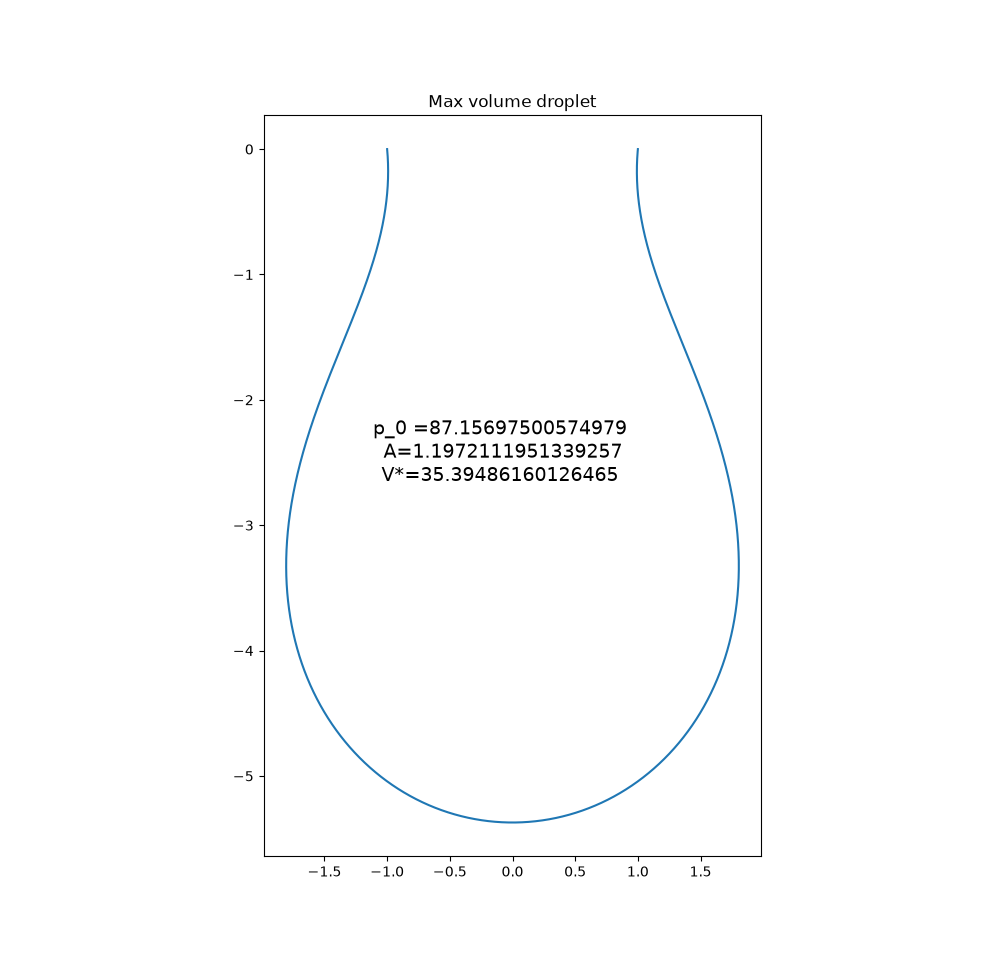
\includegraphics[width=0.45\textwidth]{max_volume_droplet.png}
        \caption{Gota com volume máximo}
    \end{figure}
\end{frame}

\begin{frame}{Pressão máxima}
    Podemos usar uma busca binária para encontrar a pressão máxima. Se o valor de $A$ estiver acima da pressão máxima, o valor do volume será maior do que $5.0$. Neste caso, diminuimos o valor máximo do intervalo e, caso contrário, aumentamos o valor mínimo do intervalo.
    \begin{figure}
        \centering
        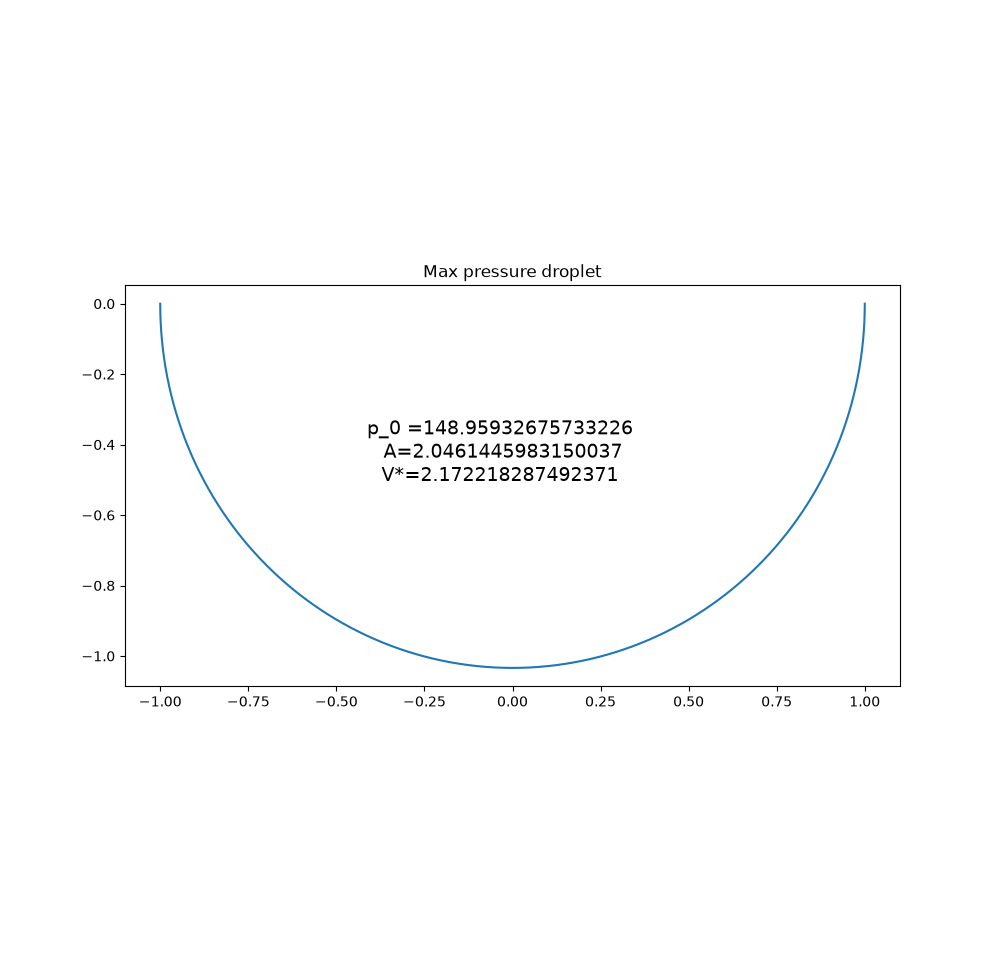
\includegraphics[trim=0cm 6cm 0cm 6cm, clip, width=0.7\textwidth]{max_press_droplet.png}
        \caption{Gota com volume máximo}
    \end{figure}
\end{frame}

\begin{frame}
    \frametitle{Teste sem gravidade}
    Note que, se $g = 0$, então $B=0$. Com isso, o PVI se torna:
    \[
        \begin{bmatrix}
            r' \\ z' \\ \theta'
        \end{bmatrix} = \begin{bmatrix}
            \cos \theta \\
            \sin \theta \\
            A - \frac{\sin \theta}{r}
        \end{bmatrix}
    \]

    Note também que, usando $d\theta = \theta' dt$: 
    \[
        r(s) - r(0) = r(s) = \int_0^s \cos(\theta(t)) dt \implies r(s)\theta'(s) =  \int_0^s \cos \theta d\theta = \sin\theta
    \]
    Logo
    \[
        \frac{\sin \theta}{r} = A  \theta' \implies \sin \theta = Ar - r\theta' = Ar - \sin \theta \implies r = \frac{2 \sin \theta}{A}
    \]
\end{frame}

\begin{frame}
    \frametitle{Teste sem gravidade}
    Substituindo esses valores na equação da derivada de $\theta$:
    \[
        \theta' = \frac{A}{2} \implies \theta(s) = \int_0^s \frac{A}{2} dt = \frac{A}{2}s
    \]
    Portanto:
    \[
        r(s) = \frac{2}{A}\sin\left( \frac{A}{2}s \right)
    \]
    \[
        z(s) = -\frac{2}{A}\cos\left( \frac{A}{2}s \right) - \frac{2}{A}
    \]
    Isso define uma bola com raio $\frac{2}{A}$ com centro $(0, -2/A)$. Logo, sem a gravidade, a solução deve ser esse círculo.
\end{frame}

\begin{frame}{Teste sem gravidade}
    \begin{figure}
        \centering
        \begin{subfigure}[b]{0.45\textwidth}
            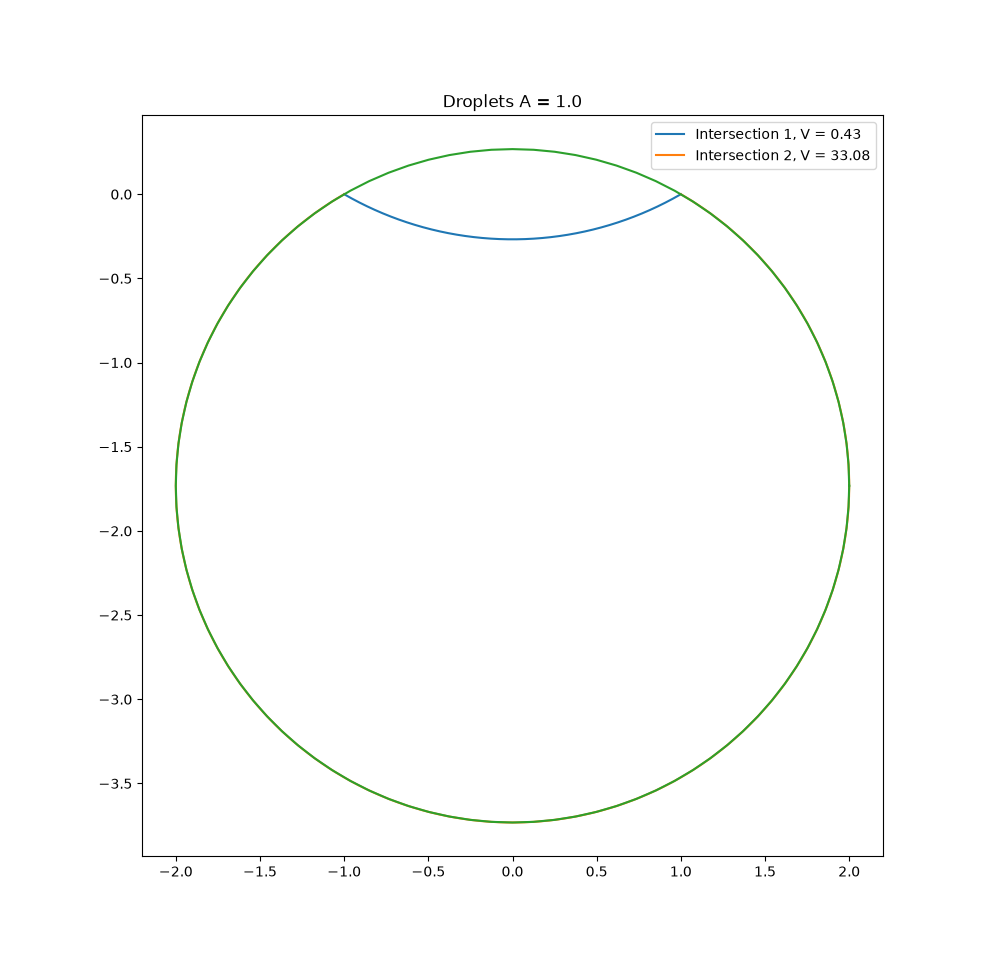
\includegraphics[width=\textwidth]{no_g_A=1.0.png}
            \caption{Comparação: Solução do PVI sem gravidade versus círculo ($A=1.0$)}
        \end{subfigure}
        \quad
        \begin{subfigure}[b]{0.45\textwidth}
            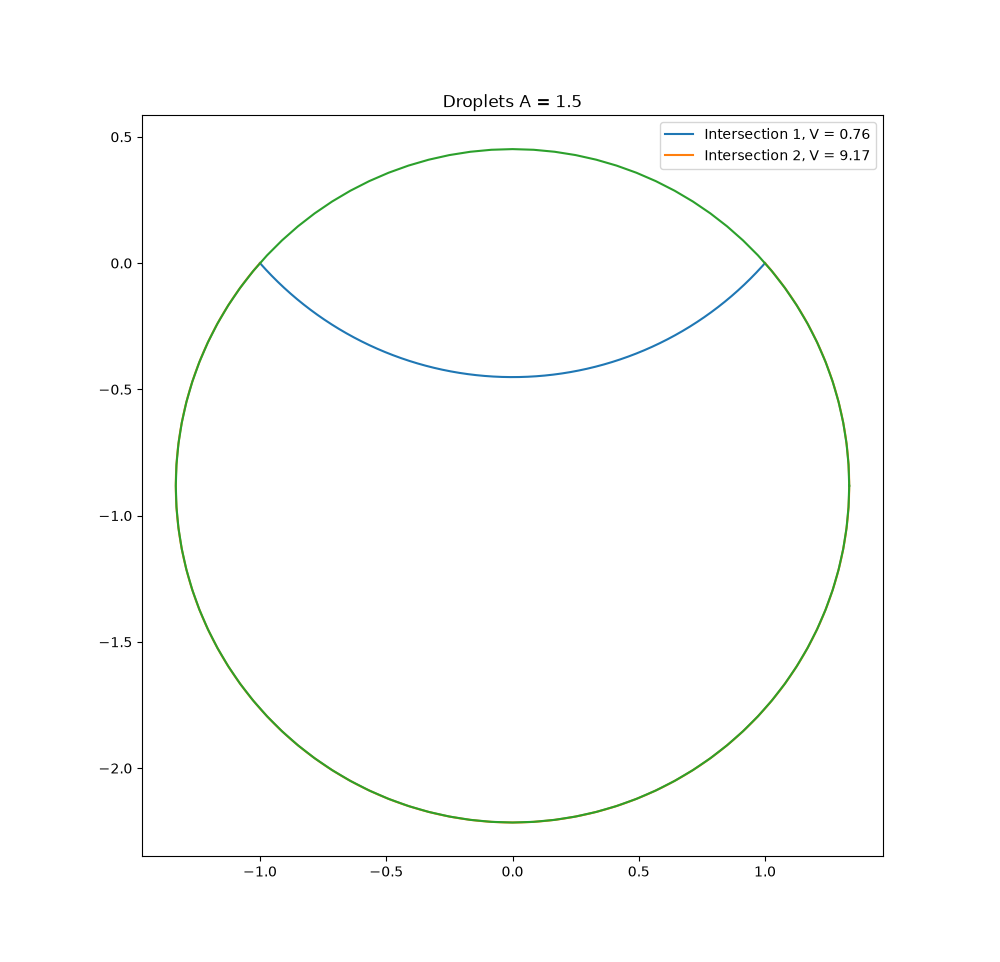
\includegraphics[width=\textwidth]{no_g_A=1.5.png}
            \caption{Comparação: Solução do PVI sem gravidade versus círculo ($A=1.5$)}
        \end{subfigure}
    \end{figure}
\end{frame}

\section{Shooting}

\begin{frame}{Método shooting}
    Dados $A_0$, $A_1$ e um volume objetivo $\hat{V}$, e os respectivos volumes mais próximos de $\hat{V}$, $V_0$ e $V_1$. Interpolamos a pressão inicial $A(V)$ pela reta:
    \[
        A(V) = A_1 + (V-V_1) \frac{A_0 - A_1}{V_0 - V_1}
    \]
    Tomamos então $A_2 = A(\hat{V})$ e fazemos o mesmo processo com $A_1$ e $A_2$. Fazemos esse processo indutivamente até que $|V_f - \hat{V}| < tol$, aqui usado $tol = 10^{-10}$
\end{frame}

\begin{frame}
    \begin{figure}
        \centering
        \begin{subfigure}[b]{0.45\textwidth}
            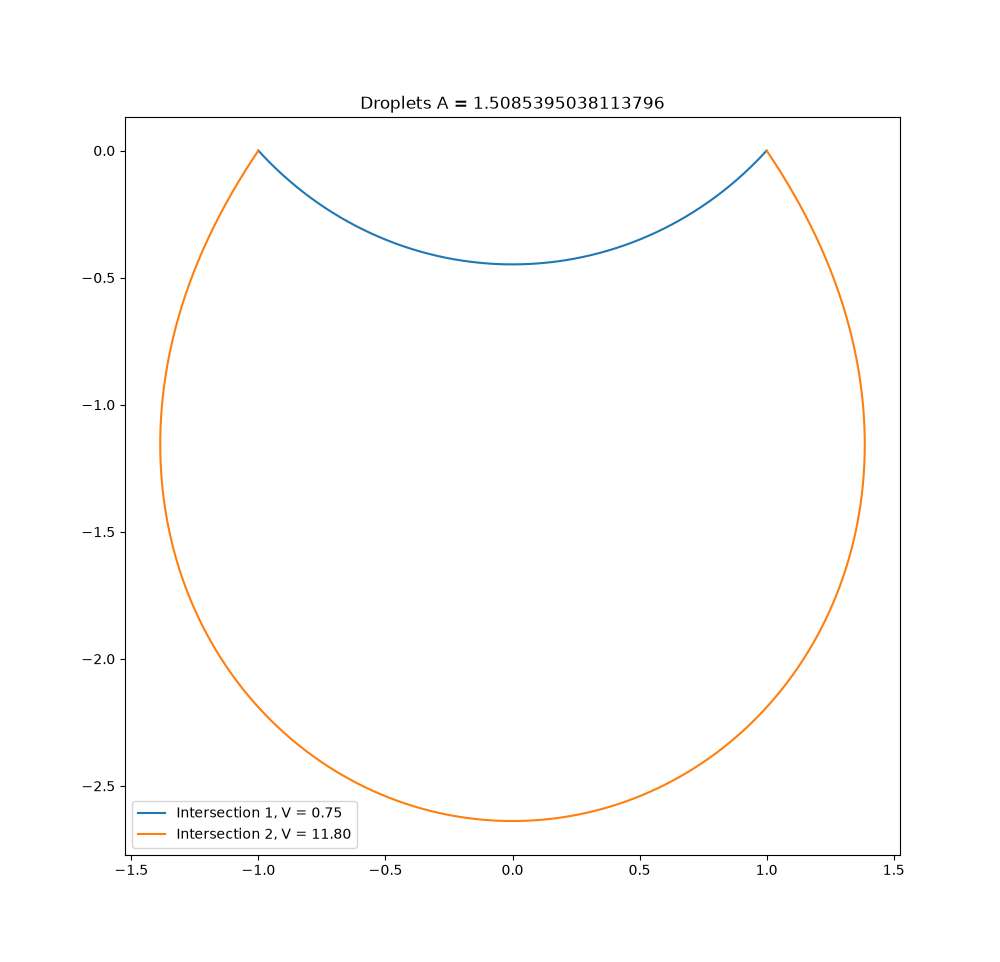
\includegraphics[width=\textwidth]{Droplet_V_1-3.png}
            \caption{Gota com volume $\frac{V^*}{3}$}
        \end{subfigure}
        \quad
        \begin{subfigure}[b]{0.45\textwidth}
            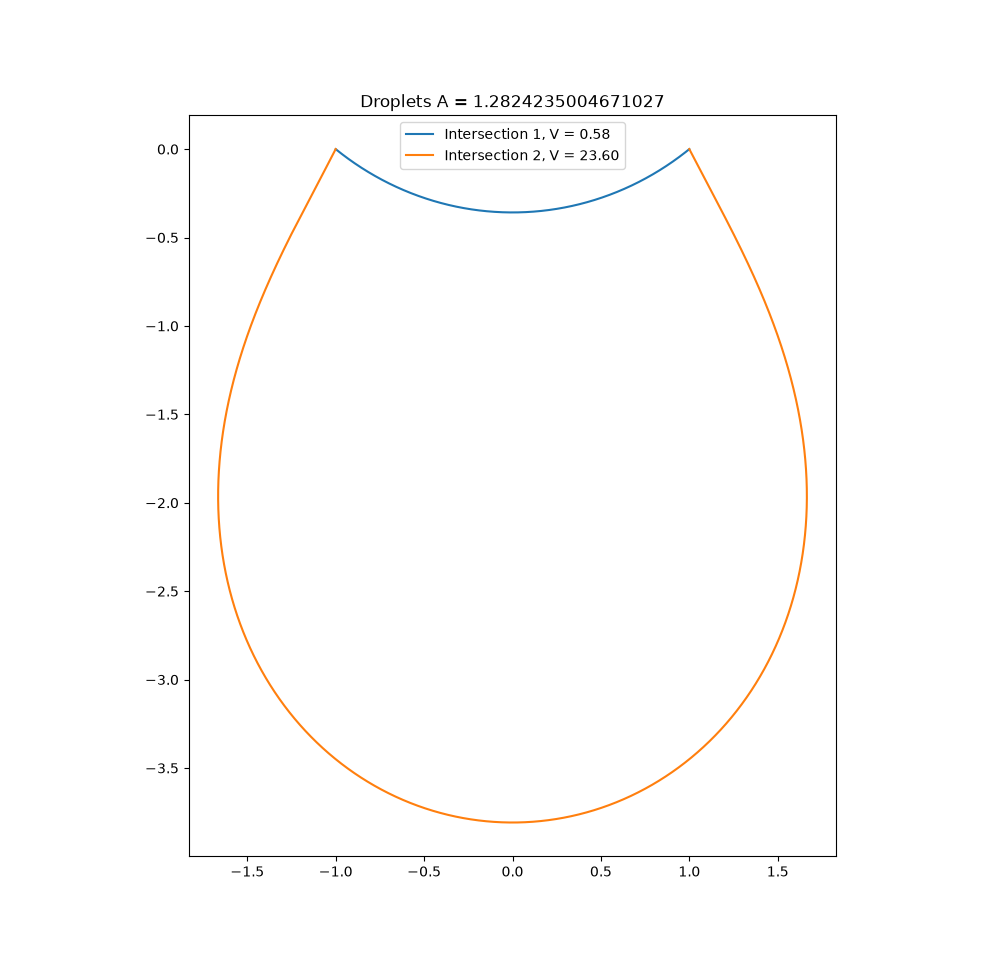
\includegraphics[width=\textwidth]{Droplet_V_2_3.png}
            \caption{Gota com volume $\frac{2V^*}{3}$}
        \end{subfigure}
    \end{figure}
\end{frame}

\begin{frame}{Várias gotas}
    \begin{figure}
        \centering
        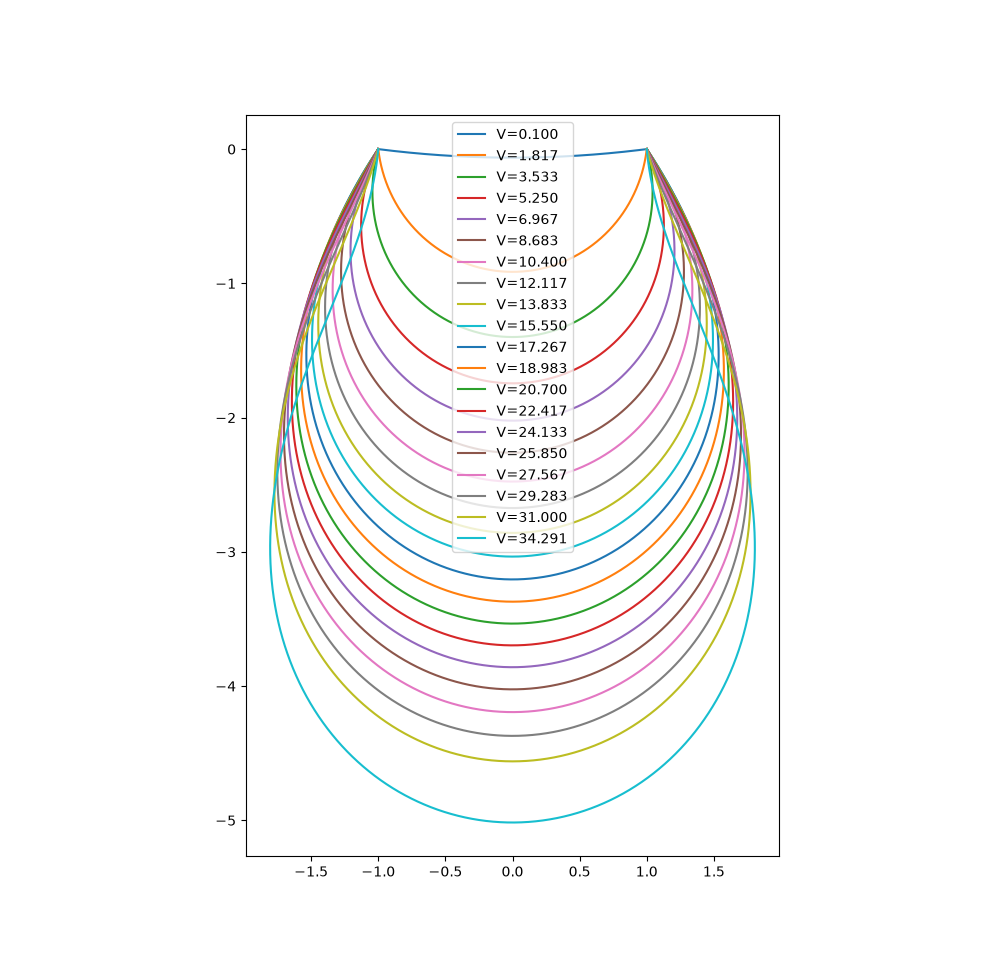
\includegraphics[width=0.7\textwidth]{Various_droplets.png}
        \caption{Gotas de diversos volumes}
    \end{figure}
\end{frame}

\end{document}